% Copyright (c) 2026 Geovana Neves. Licensed under CC BY 4.0 (https://creativecommons.org/licenses/by/4.0/). See LICENSE-AND-AUTHORSHIP.md.
%
% 01-workspaces/main.tex
%
% Guide 1 of the fts-workspace guides: the workspace, its files, running,
% and working on a Windows workstation and an HPC cluster with two
% workspaces kept together by sync. Built by ../build-all.ps1 (or
% build-all.sh) with this folder and ../shared/ as include directories.
%
% No em dashes and no en dashes. No underscores in frame or section titles
% outside \code: beamer writes titles to .nav and .toc.

\documentclass[aspectratio=169,11pt]{beamer}

\input{preamble-slides.tex}
\input{hooks-slides.tex}
\ftsinput{boxes}
\ftsinput{hooks-contract}

\usepackage[nohyphen]{underscore}

\input{info.tex}

% Table columns, ragged right so a narrow cell never hyphenates or stretches:
% P{width} for a fixed column, R for the one that takes the rest.
\newcolumntype{P}[1]{>{\RaggedRight\arraybackslash}p{#1}}
\newcolumntype{R}{>{\RaggedRight\arraybackslash}X}

\begin{document}

\guidetitleframe{1}{Workspaces}{Workspaces}
  {One tree, two workspaces, and every file in it}
  {Sources: the package pages ``The workspace and the workflow'' and
   ``Storage and sync'' [1, 2].}

\begin{frame}{Who reads what}
\begin{columns}[T]
\begin{column}{0.48\textwidth}
\begin{block}{You are going to USE the workspace}
\begin{itemize}\small
  \item Parts 1 and 2: the tree and the map.
  \item Parts 3 and 4: first time on Windows; on the cluster it is one line.
  \item Parts 5 and 6: inputs and site folders.
  \item Parts 7 and 8: choosing a workflow, and the quasi-steady rotor.
  \item Parts 9 to 11: running, what a run and its post leave.
  \item Parts 12 and 13: Windows and an HPC cluster, two workspaces and sync;
        space on disk.
  \item Parts 14 and 15: version control, and a reference.
\end{itemize}
\end{block}
\end{column}
\begin{column}{0.48\textwidth}
\begin{block}{The other guides}
\begin{itemize}\small
  \item 2: from the GUI to pyfs. \quad 3: the reference file.
  \item 4: solver setup. \quad 5: post-processing definitions.
  \item 6: fluid-structure interaction.
  \item 7: installing Python and the package on an offline machine,
        Windows and Linux. It happens once per machine.
\end{itemize}
\end{block}
\end{column}
\end{columns}
\end{frame}

\begin{frame}{Contents}
\begin{multicols}{2}
\tableofcontents
\end{multicols}
\end{frame}

% Copyright (c) 2026 Geovana Neves. Licensed under CC BY 4.0 (https://creativecommons.org/licenses/by/4.0/). See LICENSE-AND-AUTHORSHIP.md.
%
% 01-workspaces/text/01-orientation.tex

\section{One tree, two workspaces}

\begin{frame}{A workspace is a folder}
\begin{columns}[T]
\begin{column}{0.48\textwidth}
\begin{itemize}
  \item Everything a study needs is \textbf{inside one folder}: the matrix,
        the inputs it cites by name, the meshes, the results.
  \item Nothing lives in a database, a registry or somebody's head.
  \item A study moves between machines by being \textbf{opened} there.
\end{itemize}
\end{column}
\begin{column}{0.48\textwidth}
{\ftstablesize
\begin{tabular}{@{}p{0.32\linewidth}p{0.58\linewidth}@{}}
\toprule
\textbf{Machine} & \textbf{What it is for} \\
\midrule
Windows workstation & planning, one point, looking at it \\
HPC cluster & a long march, many points \\
\bottomrule
\end{tabular}}

\vspace{3mm}
{\scriptsize
main: \code{\mainworkspace}\\
cluster: \code{\clusterworkspace}\par}
\end{column}
\end{columns}
\begin{takeaway}The solver seat and the queue are both scarce, in different ways.
Use each machine for what it is good at.\end{takeaway}
\end{frame}

\begin{frame}{The path is not a preference}
\begin{center}
{\Large\bfseries\color{hanblue}\code{\mainworkspace}}\par
\vspace{1mm}{\small one agreed root, the same for everybody}
\end{center}
\begin{columns}[T]
\begin{column}{0.48\textwidth}
\begin{block}{Why}
\begin{itemize}
  \item The solver is reached by an \textbf{absolute path}.
  \item Paths are \textbf{recorded inside runs}; another root stops finding
        them months later.
\end{itemize}
\end{block}
\end{column}
\begin{column}{0.48\textwidth}
\begin{alertblock}{How it gets broken}
\begin{itemize}
  \item A workspace in \code{Documents}. Move it, do not fix it up.
  \item A mapped drive letter, \code{Z:/...}. Per user, per session.
  \item The agreed root cannot be created? \textbf{Stop and raise it.}
\end{itemize}
\end{alertblock}
\end{column}
\end{columns}
\end{frame}

\begin{frame}{What differs between the two machines}
\slidefig[0.50]{guide-one-tree-two-machines}
\begin{itemize}\small
  \item \code{inputs/hpc/h001.toml}: cluster only, how the cluster runs a job.
  \item \code{inputs/executables.local.toml}: per machine, never versioned.
  \item \code{inputs/sync-workspaces.toml}: on the main workspace, which
        brings the cluster's runs home (Part~\ref{sec:two-workspaces}).
\end{itemize}
\end{frame}

\section{The map}

\begin{frame}{The whole tree}
\slidefig[0.80]{guide-workspace-tree}
\end{frame}

\begin{frame}{NATIVE or OURS, and three writers}
\begin{columns}[T]
\begin{column}{0.44\textwidth}
\begin{block}{Two kinds of folder}
\begin{itemize}
  \item \textbf{NATIVE}: created by \pyfs{pyfs-matrix init}. Renaming one
        breaks the tool.
  \item \textbf{OURS}: added by the site (for example \code{ansa/},
        \code{builds/}, \code{docs/}). Renaming one is a team decision.
\end{itemize}
\end{block}
\end{column}
\begin{column}{0.52\textwidth}
{\ftstablesize
\begin{tabular}{@{}lp{0.62\linewidth}@{}}
\toprule
\textbf{Writer} & \textbf{Writes} \\
\midrule
You        & \code{inputs/}, \code{matriz.fs}, \code{ansa/}, \code{docs/} \\
The tool   & \code{sims/}, \code{post/}, \code{archive/}; two pproc guides in \code{inputs/pproc/} \\
The solver & inside a datapoint folder \\
\bottomrule
\end{tabular}}
\end{column}
\end{columns}
\vspace{2mm}
\begin{takeaway}You never edit anything under \code{sims/} or \code{post/}. If a
number there is wrong, an input is wrong.\end{takeaway}
\end{frame}

% Copyright (c) 2026 Geovana Neves. Licensed under CC BY 4.0 (https://creativecommons.org/licenses/by/4.0/). See LICENSE-AND-AUTHORSHIP.md.
%
% 01-workspaces/text/02-first-time.tex

\section{First time on Windows}

\begin{frame}[fragile]{Four steps before the first plan}
\begin{enumerate}
  \item \textbf{Get the workspace} into \code{\mainworkspace}: a checkout from
        your version control, or a copy of the study's folder.
  \item \textbf{Install} Python 3.12 or newer and the package in a virtual
        environment (offline machine: Guide 7):
\begin{lstlisting}[style=ftsbase]
py -3.12 -m venv .venv
.venv\Scripts\activate
pip install pyflightstream==(*@\pkgversion@*)
\end{lstlisting}
  \item \textbf{Point at the solver} in \code{inputs/executables.local.toml},
        forward slashes, absolute path.
  \item \textbf{Read the boundary order off the mesh}, never type it:
\begin{lstlisting}[style=ftsbase]
pyfs-matrix inventory inputs/geometries/<mesh>/<mesh>.fsm
\end{lstlisting}
\end{enumerate}
\end{frame}

\begin{frame}[fragile]{Plan first, always}
\begin{lstlisting}[style=ftsbase]
pyfs-matrix plan matriz.fs --workspace . --fs-version 26.123
pyfs-matrix plan matriz.fs --workspace . --fs-version 26.123 --cost
\end{lstlisting}
\begin{columns}[T]
\begin{column}{0.48\textwidth}
\begin{itemize}
  \item Spends \textbf{no seat and no queue}.
  \item Writes the receipt \pyfs{run} refuses to start without.
  \item The receipt carries the matrix digest: an edit between plan and run
        is visible.
\end{itemize}
\end{column}
\begin{column}{0.48\textwidth}
\begin{itemize}
  \item \code{--cost}: mesh size, run type, steps, processors, and an
        \emph{expected} time.
  \item The time is an extrapolation from this workspace's own runs, and says
        so. No comparable run, no number.
  \item It warns when the points still to run may not fit on the disk
        (Part~\ref{sec:storage}).
\end{itemize}
\end{column}
\end{columns}
\end{frame}

\begin{frame}[fragile]{A healthy first run}
\small The rotor row states \code{LAST\_REVS\_AVG: 1}; its flight condition
lists Mach, alpha, beta and advance ratio, in that order.
\begin{lstlisting}[style=ftsbase]
pyfs-matrix run matriz.fs --workspace . --fs-version 26.123

  -> fts-workspace/sim_0001/M144AL+000BE+000J+100  [unsteady_rotor]  building and running
     fts-workspace/sim_0001/M144AL+000BE+000J+100  CONVERGED
  ...
sweep table: <workspace>\post\matriz\campaign_sweep.csv
\end{lstlisting}
\begin{itemize}
  \item Each line names the \textbf{run id}; the point tag ends it.
  \item The last line is the table most people open.
  \item Read \code{skipped}: it may name an inapplicable reduction or missing
        data needed by a product.
\end{itemize}
\end{frame}

\section{The cluster}

\begin{frame}[fragile]{Using it is one line}
\begin{lstlisting}[style=ftsbase]
source (*@\clusterroot@*)/bin/(*@\envname@*)-env
\end{lstlisting}
\begin{columns}[T]
\begin{column}{0.48\textwidth}
\begin{itemize}
  \item At the top of a session \textbf{or of a job script}.
  \item Nobody installs, nobody builds an environment, nobody asks
        permission.
  \item One environment for everybody, which is what makes two people's
        results comparable.
\end{itemize}
\end{column}
\begin{column}{0.48\textwidth}
\begin{alertblock}{An alias is not available to a job}
A job script does not expand aliases and fails after the queue wait with
\code{command not found}. Keep an alias as a convenience, never as the
mechanism.
\end{alertblock}
\end{column}
\end{columns}
\end{frame}

\begin{frame}[fragile]{Leaving the environment}
% \relax first: a brace group right after the title is read as a subtitle.
\relax
{\ftstablesize
\begin{tabular}{@{}ll@{}}
\toprule
\textbf{You sourced} & \textbf{To leave} \\
\midrule
\code{py-venv/\envname/bin/activate} & \code{deactivate} \\
\code{bin/\envname-env} & a new shell, or \code{exit} \\
\bottomrule
\end{tabular}}

\vspace{2mm}
The shared file only puts one folder at the front of \code{PATH}. To keep the
shell open, take it off again:
\begin{lstlisting}[style=ftsbase]
export PATH=${PATH#(*@\clusterroot@*)/py-venv/(*@\envname@*)/bin:}
which pyfs-matrix     # must no longer name py-venv/(*@\envname@*)
\end{lstlisting}
\begin{takeaway}Leave one environment before sourcing another. \code{which
pyfs-matrix} says which one you are in.\end{takeaway}
\end{frame}

\begin{frame}{Installing is another guide}
\begin{itemize}
  \item Python 3.12, the wheels and the shared environment are installed
        \textbf{once, by one person}, from a connected machine: Guide 7,
        \emph{Python environment for offline machines}.
  \item Everybody else sources one line, above.
\end{itemize}
\end{frame}

% Copyright (c) 2026 Geovana Neves. Licensed under CC BY 4.0 (https://creativecommons.org/licenses/by/4.0/). See LICENSE-AND-AUTHORSHIP.md.
%
% 01-workspaces/text/03-inputs.tex

\section{The input files}

\begin{frame}{The row names things, the files define them}
\slidefig[0.62]{guide-inputs-into-run}
\begin{takeaway}By name, never by path: \code{REF}, \code{SET} and \code{PPROC}
carry a file stem, \code{GEOMETRY} names the mesh. That is what lets one matrix
drive two workspaces.\end{takeaway}
\end{frame}

\begin{frame}{\code{matriz.fs}: nineteen columns}
% \relax first: a brace group right after the title is read as a subtitle.
\relax
{\ftstablesize
\begin{tabular}{@{}ll@{}}
\toprule
\textbf{Group} & \textbf{Columns} \\
\midrule
identity: does it run at all & \code{POL}, \code{HIDDEN}, \code{RUN} \\
what it is     & \code{AIRCRAFT}, \code{CONFIGURATION}, \code{DESCRIPTION} \\
what it flies  & \code{FLIGHT\_CONDITION}, \code{SWEEP\_VALUES} \\
what it cites  & \code{GEOMETRY}, \code{REF}, \code{SET}, \code{PPROC} \\
how it solves  & \code{SYMMETRY}, \code{SYMMETRY\_LOADS}, \code{NCPUS}, \code{WALLTIME}, \code{FS\_BUILD} \\
what builds it & \code{WORKFLOW}, \code{VAR\_NAMES\_VALUES} \\
\bottomrule
\end{tabular}}
\vspace{3mm}
\begin{itemize}
  \item A key \textbf{every row} must answer is a column; a key only some rows
        need goes in the free cell, \code{VAR\_NAMES\_VALUES}.
  \item \code{-} means \emph{stated nothing}, so it cannot be confused with a
        truncated line.
\end{itemize}
\end{frame}

\begin{frame}[fragile]{One POL, once, in the whole workspace}
\begin{itemize}
  \item \code{POL} names \code{sims/sim\_<POL>} and the run ids, so it appears
        \textbf{once across every matrix} of the workspace, \code{RUN = 0}
        rows included.
  \item \pyfs{plan} refuses a repeated POL and lists where it appears.
\end{itemize}
\begin{lstlisting}[style=ftsbase]
pyfs-matrix plan matriz.fs --workspace . --fs-version 26.123 --update-ids
\end{lstlisting}
\begin{itemize}
  \item \code{--update-ids} gives each repeated row of \emph{this} matrix the
        next free POL above every POL, run record and \code{sims/} folder
        \textbf{it can see}.
\end{itemize}
\begin{alertblock}{It writes the matrix before planning}
The renumbering stays written even if the plan then refuses. Commit first, so
the change is one diff you can read.
\end{alertblock}
\end{frame}

\begin{frame}[fragile]{The free cell: move, turn, raw}
\begin{lstlisting}[style=ftsbase]
TRANSLATE: {DISTANCE: 0.05 / AXIS: PUSHER_SMRP-X / ALIAS: PUSHER}
ROTATE:    {ANGLE: 3 / AXIS: PUSHER_SMRP-Y / ALIAS: PUSHER}
RAW:       {COMMAND: SOLVER_SET_ITERATIONS 350 / BEFORE: init}
\end{lstlisting}
\begin{columns}[T]
\begin{column}{0.48\textwidth}
\begin{itemize}\small
  \item \code{TRANSLATE}: metres, along \textbf{one} axis; a diagonal
        is two records.
  \item \code{ROTATE}: degrees, about one axis.
  \item \textbf{Every translation comes before every rotation}, whatever the
        order written.
  \item One row is one position: neither is swept.
\end{itemize}
\end{column}
\begin{column}{0.48\textwidth}
\begin{alertblock}{What to know before using it}
\begin{itemize}\small
  \item The alias's frames move with it; \code{<ALIAS>\_SMRP\_ORIGINAL} keeps
        the hub where it was.
  \item A moved part \textbf{comes away} from what it touches: the junction
        is open.
  \item The distance is read in metres; keep the meshes in metres.
\end{itemize}
\end{alertblock}
\end{column}
\end{columns}
\end{frame}

\begin{frame}[fragile]{The flight condition: constraints on one flow state}
\begin{columns}[T]
\begin{column}{0.50\textwidth}
\begin{lstlisting}[style=ftsbase]
FLIGHT_CONDITION: MACH:0.20, REmi:5.5
FLIGHT_CONDITION: TASmps:68.08, ALTFT:10000, dISA:5
\end{lstlisting}
{\ftstablesize
\begin{tabular}{@{}>{\raggedright\arraybackslash}p{0.16\linewidth}>{\raggedright\arraybackslash}p{0.24\linewidth}>{\raggedright\arraybackslash}p{0.46\linewidth}@{}}
\toprule
\textbf{Key} & \textbf{Unit} & \textbf{Constrains} \\
\midrule
\code{MACH}   & none & velocity, by the state's speed of sound \\
\code{TASmps} & m/s & velocity, directly \\
\code{REmi}   & \textbf{millions} & density \\
\code{ALTFT}  & \textbf{feet} & pressure and temperature \\
\code{dISA}   & \textbf{Celsius, a delta} & temperature \\
\bottomrule
\end{tabular}}
\end{column}
\begin{column}{0.46\textwidth}
\begin{itemize}\small
  \item The keys decide what is solved for: the first line solves the
        \textbf{density}, the second is an atmosphere point whose Reynolds
        number follows [5, 7, 8].
  \item Exactly one of \code{MACH} or \code{TASmps}. \code{REmi} needs the
        row's \code{REF}: a Reynolds number has no meaning without a length.
  \item Five keys \textbf{pin} the fluid (\code{RHOkgm3}, \code{MUPas},
        \code{ASMPS}, \code{TK}, \code{PPA}), on the row or in the setup's
        \code{[flight\_condition]}.
  \item A rotor: \(V = J\,(\mathrm{RPM}/60)\,D\); state two of the three.
  \item The set is closed: an unknown key is refused, never ignored.
\end{itemize}
\end{column}
\end{columns}
\end{frame}

\begin{frame}[fragile]{A matrix from an older layout}
\begin{lstlisting}[style=ftsbase]
pyfs-matrix upgrade matriz.fs              # to standard output: read the diff
pyfs-matrix upgrade matriz.fs --in-place   # then write it
\end{lstlisting}
\begin{itemize}\small
  \item A matrix written under an earlier layout is recognised by its header
        and \textbf{refused rather than misread}; \code{upgrade} converts it.
        It needs no recipe, no build and no executable.
  \item A sweep code becomes the word \code{sweep} where the value would be:
        \code{AL} becomes \code{ALPHA:sweep}. A row that varies both angles is
        refused by name: it is one row per sideslip, each with its own POL.
  \item \textbf{The values move across verbatim; the result may not.} A
        Reynolds number that was only recorded becomes a constraint that
        solves for density, so the upgraded row emits a fluid state it never
        emitted before. To keep the old behaviour, drop \code{REmi} and let the
        Reynolds number follow.
\end{itemize}
\end{frame}

\begin{frame}[fragile]{\code{r001.toml}: what things are called (Guide 3)}
\begin{columns}[T]
\begin{column}{0.46\textwidth}
\begin{lstlisting}[style=ftsbase]
area_m2 = 19.502
chord_m =  1.322
span_m  = 15.059
[moment_point]
x_m = 0.0

[aliases]
airframe = ["Spinner","Nacelle"]

[PUSHER]
kind = "rotor"
axis = "X"
diameter_m = 1.80
blade1 = { azimuth_deg = 0, zero = "Y" }
families_blades = ["Blade1", "Blade2"]
\end{lstlisting}
{\tiny\color{SoftGray} The template's synthetic numbers; a study replaces every one.}
\end{column}
\begin{column}{0.50\textwidth}
\begin{itemize}\small
  \item Reference lengths and the moment point divide every coefficient.
  \item An \textbf{alias} is a word rows, groups and plots cite.
  \item A rotor block creates \code{<NAME>\_SMRP}, \code{<NAME>\_RMRP} and
        \code{<NAME>\_RMRP<k>}.
  \item The blade count is the length of \code{families\_blades}.
\end{itemize}
\begin{alertblock}{The failure nothing refuses}
A wrong moment point gives plausible, wrong coefficients. Get it right by
reading.
\end{alertblock}
\end{column}
\end{columns}
\end{frame}

\begin{frame}[fragile]{Setup, post-processing and profiles}
\begin{columns}[T]
\begin{column}{0.32\textwidth}
\begin{block}{\code{s001.toml}}
\small How hard to solve and when to stop. Multiplatform. A command every row
needs goes in its \code{[[raw]]} table.
\end{block}
\end{column}
\begin{column}{0.32\textwidth}
\begin{block}{\code{p001.toml}}
\small What the run exports. The log is declared \textbf{last}: its presence
says the run finished. The \code{.fsm} of every point is always saved;
\code{simulation = false} is refused.
\end{block}
\end{column}
\begin{column}{0.32\textwidth}
\begin{block}{\code{inputs/profiles/}}
\small Probe surveys a \code{[[probes]]} entry cites by \code{points\_file}.
Resolved to an absolute path; a missing file is refused at plan.
\end{block}
\end{column}
\end{columns}
\begin{lstlisting}[style=ftsbase]
[[probes]]
frame = "MRP"
parameters = ["VELOCITY"]
points_file = "disk_survey.txt"     # inputs/profiles/disk_survey.txt
\end{lstlisting}
\end{frame}

\begin{frame}[fragile]{The solver path and the cluster profile}
\begin{columns}[T]
\begin{column}{0.48\textwidth}
\begin{block}{Two files, one sentence}
\small \code{executables.toml} is about the \textbf{study} and is versioned.
\code{executables.local.toml} is about the \textbf{machine} and is not.
\end{block}
\begin{alertblock}{Exactly one HPC profile}
\small More than one in \code{inputs/hpc/} is refused: there is no selector.
\end{alertblock}
\end{column}
\begin{column}{0.48\textwidth}
\begin{lstlisting}[style=ftsbase]
# inputs/hpc/h001.toml
[descriptor.fields]
version = "{fs_build_alias}"

[builds]
"26.123" = "26.1"
\end{lstlisting}
\begin{itemize}\small
  \item The row keeps the build, the profile gives the scheduler's word.
  \item A declaration, not a check: the build number in the collected log is
        the proof.
\end{itemize}
\end{column}
\end{columns}
\end{frame}

\begin{frame}[fragile]{The row states its window}
\begin{itemize}
\item \code{unsteady\_rotor}: \code{LAST\_REVS\_AVG}, in revolutions;
fractions are accepted.
\item \code{unsteady}: \code{LAST\_ITERS\_AVG}, in solver steps.
\item With no window key, \pyfs{plan} refuses the row. \code{WINDOW\_*}
keys are refused, naming the key to write.
\end{itemize}
\small Temporal fragments for the free cell, beside the other required keys:
\begin{lstlisting}[style=ftsbase]
DELTA_THETA: 5 / REVOLUTIONS: 4 / LAST_REVS_AVG: 1
DELTA_TIME: 0.01 / TIME_ITERATIONS: 100 / LAST_ITERS_AVG: 20
\end{lstlisting}
\begin{alertblock}{One declaration of each attitude}
\small \code{ALPHA} or \code{BETA} in both \code{FLIGHT\_CONDITION} and
\code{VAR\_NAMES\_VALUES} is refused, even if the values agree.
\end{alertblock}
\end{frame}

\begin{frame}[fragile]{Groups and optional pproc tables}
\begin{columns}[T]
\begin{column}{0.47\textwidth}
\begin{lstlisting}[style=ftsbase]
[groups]
PUSHER = "PUSHER"
AIRFRAME = "airframe"
TOTAL = "all"

[phase_locked]
min_revolutions = 4.0
last_revolutions_avg = 2.0

[products]
superfile_format = "legacy_polar"
\end{lstlisting}
\end{column}
\begin{column}{0.49\textwidth}
\begin{itemize}\small
\item One alias as a string. A list is refused with the
one-alias line to write; several members go in the reference's \code{[aliases]}.
\item \code{[phase\_locked]}: one row per azimuth across revolutions;
no declaration keeps the passage series.
\item \code{[equations]} and \code{[glossary]} bind too: derived
columns at post, named \code{<NAME>\_<alias>}; equations may chain.
\item Fixed-width super file: sixteen characters per field; \code{csv}
remains the default.
\end{itemize}
\end{column}
\end{columns}
\end{frame}

\begin{frame}[fragile]{Names and plot-group declarations}
\begin{lstlisting}[style=ftsbase]
[names]
CL_MRP_TOTAL = "CL_TOTAL"
\end{lstlisting}
\begin{itemize}\small
\item Requires that plotted source column. The whole dictionary applies or
none does; missing sources and occupied destinations produce a \code{\#names}
skip. \code{CL} is already the native last-step health check.
\item Applied after axes and equations to the unsteady polar, time average
and passage series. Plots, per-blade and azimuthal headings retain their names.
\item Plot-group names: letters, digits, underscores and bare
\code{\{family\}} only. No spaces, format spec or conversion.
\item Ambiguous names cannot supply rotor histories or global axis blocks.
\item \code{VARIABLES.md} and \code{WRITING-EQUATIONS.md} are generated in
\code{inputs/pproc/} by init, plan and post; commit or ignore them.
\end{itemize}
\end{frame}

\begin{frame}[fragile]{A mesh file, OBJ or STL}
\begin{columns}[T]
\begin{column}{0.50\textwidth}
\begin{lstlisting}[style=ftsbase]
# wing/wing.boundaries.toml, beside wing.obj
boundaries = ["Wing"]      # OBJ: from its groups

[import]
units = "METER"            # the FILE's unit

[trailing_edges]
file = "wing.te.txt"       # points file
\end{lstlisting}
\begin{alertblock}{Export the mesh in metres}
\small On 26.124 a wing OBJ in millimetres, its trailing edge detected,
solved as the same wing in metres to the print [3]: \code{IMPORT}
converts. The file route in millimetres, and every other build, are not
measured.
\end{alertblock}
\end{column}
\begin{column}{0.46\textwidth}
\begin{itemize}\small
  \item \code{GEOMETRY: wing.obj}, like a \code{.fsm}. The script starts a
        new simulation, imports in the stated unit, then works in metres.
  \item No \code{[import]}: refused at plan. An OBJ with no sidecar gets
        one from the plan, its \code{boundaries} read from the file's groups.
        \textbf{Still by hand}: the \code{[import]} unit, the
        trailing edge, and an STL's names, where a name in the wrong place
        cites the wrong surface.
  \item \code{[[import.operations]]}: scale, rename, mirror, translate,
        rotate, in the order written.
\end{itemize}
\end{column}
\end{columns}
\end{frame}

\begin{frame}[fragile]{The trailing edge, by file}
\begin{lstlisting}[style=ftsbase]
METER                                   # the unit of the points
0.216872113,-0.002159825,0.223199974    # one MID-POINT of an edge per line
\end{lstlisting}
\begin{itemize}\small
  \item \textbf{The default route.} Every point is checked against the mesh at
        plan; the first one off an edge is refused by line and position.
  \item The run writes the node file in metres, imports it with
        \code{IMPORT\_WAKE\_EDGES\_FROM\_FILE}, and compares the solver's count
        with the points: a difference is \code{FAILED\_SCRIPT}. A point that
        misses an edge is otherwise \textbf{silent}.
  \item \textbf{26.124 only} [3]. The row must export its log.
  \item Detection is the second route, written in full: \code{detect = "auto"},
        or by surface with a sweep angle.
  \item \code{BASE\_REGIONS} names the \textbf{base}, not the body [3].
\end{itemize}
\end{frame}

\begin{frame}{A public airframe to practise on}
\begin{columns}[T]
\begin{column}{0.54\textwidth}
\begin{itemize}\small
  \item The SMI airframe geometry [9] is published as IGES components: the
        fuselage, the nacelles with their pylons, the lifting surfaces, and
        the wing-body geometry they share. Each component is whole, so
        intermediate configurations can be built from it.
  \item It carries \textbf{no propeller}. Any rotor is added by the user and
        placed by a rotor block of the reference (Guide 3), from any
        propeller geometry the user holds.
  \item Mesh it with the site's mesher, export OBJ \textbf{in metres}, and
        write its \code{<stem>.boundaries.toml} beside it: the route of the
        two previous frames.
\end{itemize}
\end{column}
\begin{column}{0.42\textwidth}
\begin{block}{Its licence}
\small CC BY-NC 4.0: credit the record, no commercial use. Cite it as [9]
wherever a result uses it.
\end{block}
\begin{takeaway}A first workspace on a known public geometry makes a
mistake visible before it costs a campaign.\end{takeaway}
\end{column}
\end{columns}
\end{frame}

\begin{frame}[fragile]{Every key in one generated page, and an optional workbook}
\begin{columns}[T]
\begin{column}{0.48\textwidth}
\begin{block}{\code{inputs/INPUTS.md} and \code{inputs/input\_template.md}}
\begin{itemize}\small
  \item \code{INPUTS.md} lists every key an input may state: the row by run
        type, the setup, the pproc, the reference, the sidecar. Each says what
        it sets, its unit or values and the command it reaches.
  \item \code{input\_template.md} shows every input \textbf{file}, one
        complete example per kind, each one a file the package reads as it
        stands.
  \item Both are \textbf{generated} by \pyfs{init}, \pyfs{plan} and
        \pyfs{post}; never edit them.
\end{itemize}
\end{block}
\end{column}
\begin{column}{0.48\textwidth}
\begin{block}{An Excel workbook, if you want one [6]}
\small An ordinary \code{.xlsx}, no macros. Python creates it and
synchronises saved files in both directions, always as a preview first, then
an apply:
\begin{lstlisting}[style=ftsbase,basicstyle=\ttfamily\tiny]
pip install "pyflightstream[excel]"
python -m pyflightstream.workspace.excel preview
   <book>.xlsx --workspace . --direction read
   --batch read-preview.json
python -m pyflightstream.workspace.excel apply
   read-preview.json
\end{lstlisting}
The ASCII matrix stays the record; the workbook is an editor.
\end{block}
\end{column}
\end{columns}
\end{frame}

\section{Site folders}

\begin{frame}{\code{ansa/}, \code{builds/}, \code{docs/}}
\begin{columns}[T]
\begin{column}{0.32\textwidth}
\begin{block}{\code{ansa/}}
\small The mesh scripts. The script is versioned, the mesh is not.
\end{block}
\end{column}
\begin{column}{0.32\textwidth}
\begin{block}{\code{builds/}}
\small One folder per solver build number.
\end{block}
\end{column}
\begin{column}{0.32\textwidth}
\begin{block}{\code{docs/}}
\small What a second person needs to repeat the first one's work: these
guides, the install notes.
\end{block}
\end{column}
\end{columns}
\vspace{2mm}
\begin{block}{Adding a build, in order}
\small \textbf{1} copy into its own folder \quad \textbf{2} register in
\code{executables.toml} \quad \textbf{3} point your local file at it, and add its
\code{[builds]} line on the cluster \quad \textbf{4} plan one row and read the
build number in its log. \textbf{Keep the old build.}
\end{block}
\end{frame}

% Copyright (c) 2026 Geovana Neves. Licensed under CC BY 4.0 (https://creativecommons.org/licenses/by/4.0/). See LICENSE-AND-AUTHORSHIP.md.
%
% 01-workspaces/text/07-workflows.tex
%
% The workflows part: which run type a row takes, what each costs, and the
% quasi-steady rotor in depth. Read from cases/workflows.py (the registered
% keys), cases/qsteady.py (clocking, validity), docs/workspace-and-workflows.md
% ("The quasi-steady rotor"), reports/RPT-089 (the measurements) and the
% owner's decisions of 0.30.0 for --inflow-fft. The figures are drawn by
% figures/qsteady_reduced_frequency.py on the package's generic test blade.
%
% The count nP is the BLADE's: how many times one blade meets the same
% perturbation in one revolution. Never the blade-passing N P of a fixed
% surface, never the rotor-total balance where only multiples of N P survive.

\section{Choosing a workflow}

\begin{frame}{Four workflows, five ways to solve a row}
\relax % a body opening with a brace group would be read as the frame subtitle
{\ftstablesize\renewcommand{\arraystretch}{1.12}
\begin{tabularx}{\linewidth}{@{}P{0.17\linewidth}P{0.25\linewidth}RP{0.14\linewidth}@{}}
\toprule
\textbf{\code{WORKFLOW}} & \textbf{What is solved} & \textbf{When to use it} & \textbf{Cost} \\
\midrule
\code{steady} & one converged steady solve per point; a sweep is one job &
  a body in a steady flow: polars, sweeps, a fixed wing (FSI with its own
  weight) & seconds per point \\
\code{unsteady} & a march in physical time, nothing turning &
  a flow that changes in time without a rotor: a manoeuvre rate, a start-up,
  a fixed wing coupled per step & minutes \\
\code{unsteady\_rotor} & the blades turn, the wake is shed in time &
  the reference for any rotor: installed, interacting, several rotors, a
  time history, the in-plane loads & minutes to hours \\
\code{qsteady\_rotor}, sector & one blade held still, periodic copies, the
  free stream turning & an isolated, axisymmetric rotor in an inflow the same
  at every azimuth; blade FSI with centrifugal loads & seconds \\
\code{qsteady\_rotor}, wheel & every blade held still; one steady solve per
  clocking, averaged & the same rotor at an angle or in a custom inflow, when
  thrust and torque are what matter & seconds per clocking \\
\bottomrule
\end{tabularx}}
\par\vspace{1mm}
{\scriptsize Every row names its workflow in the \code{WORKFLOW} column; a key
another workflow registers is refused by name at \pyfs{plan}. Costs are orders
of magnitude on one workstation, measured on a six-blade research propeller
[14].\par}
\end{frame}

\begin{frame}{A decision chart}
\centering
\begin{adjustbox}{max width=\linewidth, max totalheight=0.76\textheight}
\begin{tikzpicture}[
  q/.style={draw=CourseBlue, fill=CourseBlue!6, rounded corners=1.5mm,
    align=center, font=\scriptsize, inner sep=1.3mm, text width=5.2cm},
  a/.style={draw=CourseGold, fill=CourseGold!15, align=center,
    font=\scriptsize\ttfamily, inner sep=1.2mm, minimum width=3.3cm},
  e/.style={-{Stealth[length=1.8mm]}, thick, CourseBlue},
  l/.style={font=\tiny, text=SoftGray, fill=white, inner sep=0.5mm},
  n/.style={font=\tiny, text=SoftGray, align=left}]
\node[q] (q1) at (0,0) {Does a rotor turn in the row?};
\node[q] (q2) at (0,-1.45) {An isolated, axisymmetric rotor, and nothing
  else in the flow?};
\node[q] (q3) at (0,-2.9) {Does the inflow vary around the disc (an angle of
  attack or sideslip, an azimuthal custom field)?};
\node[q] (q4) at (0,-4.35) {Are thrust and torque the answer, and \(k\) small
  over most of the span?};
\node[a] (a1) at (6.0,0) {steady {\normalfont or} unsteady};
\node[n, right=1.5mm of a1] {unsteady when the flow\\changes in time};
\node[a] (a2) at (6.0,-1.45) {unsteady\_rotor};
\node[n, right=1.5mm of a2] {an airframe, several\\rotors, a wing nearby};
\node[a] (a3) at (6.0,-2.9) {qsteady\_rotor, sector};
\node[n, right=1.5mm of a3] {an inflow varying with the\\radius alone; FSI allowed};
\node[a] (a4) at (6.0,-4.35) {qsteady\_rotor, wheel};
\node[n, right=1.5mm of a4] {\code{PASSAGE\_POSITIONS: k},\\mandatory};
\node[a] (a5) at (0,-5.65) {unsteady\_rotor};
\node[n, right=1.5mm of a5] {in-plane loads, a history, a large \(k\)};
\draw[e] (q1) -- node[l] {no} (a1);
\draw[e] (q1) -- node[l] {yes} (q2);
\draw[e] (q2) -- node[l] {no} (a2);
\draw[e] (q2) -- node[l] {yes} (q3);
\draw[e] (q3) -- node[l] {no} (a3);
\draw[e] (q3) -- node[l] {yes} (q4);
\draw[e] (q4) -- node[l] {yes} (a4);
\draw[e] (q4) -- node[l] {no} (a5);
\end{tikzpicture}
\end{adjustbox}
\par\vspace{1mm}
{\scriptsize \(k\) is the blade's 1P reduced frequency (Part ``the quasi-steady
rotor''); \pyfs{plan} prints it for every wheel point.\par}
\end{frame}

\begin{frame}{\code{steady} and \code{unsteady}}
\begin{columns}[T]
\begin{column}{0.48\textwidth}
\begin{block}{\code{steady}}
\small One converged solve per point; an \code{ALPHA:sweep} or
\code{BETA:sweep} row is one job, every point starting cold unless
\code{COLD\_START: false}. The polar, the super file and the sections are
instants of the last iteration. A custom inflow (\code{FREESTREAM}) or a
free-stream rate (\code{roll\_rate}, \code{pitch\_rate}, \code{yaw\_rate})
is still one steady solve.
\end{block}
\end{column}
\begin{column}{0.48\textwidth}
\begin{block}{\code{unsteady}}
\small A march of \code{TIME\_ITERATIONS} steps of \code{DELTA\_TIME}, and
the window it is averaged over, \code{LAST\_ITERS\_AVG}, which the row must
state. Nothing turns but the free stream; a rotor is
\code{unsteady\_rotor}'s. The products are averages over the window, and the
history is kept.
\end{block}
\end{column}
\end{columns}
\begin{takeaway}The window belongs to the row, not to the pproc: changing it
is a new \pyfs{post}, never a new run (Guide 5).\end{takeaway}
\end{frame}

\begin{frame}{\code{unsteady\_rotor}: the reference, and its price}
\begin{columns}[T]
\begin{column}{0.52\textwidth}
\begin{itemize}\small
  \item The blades turn at \code{RPM} (or from \code{ADVANCE\_RATIO}), about
        the rotor block's axis, with its hand; the step is \code{DELTA\_THETA}
        degrees or \code{DELTA\_TIME}, the length \code{REVOLUTIONS} or
        \code{TIME\_ITERATIONS}, and \code{LAST\_REVS\_AVG} is mandatory.
  \item The only workflow for a rotor on an airframe, for several rotors
        (\code{MOTIONS}), for the time history and phase-locked products, and
        the one to trust for the in-plane loads.
  \item FSI is refused on it in this release (Guide 6).
\end{itemize}
\end{column}
\begin{column}{0.44\textwidth}
\begin{alertblock}{A few revolutions are not a developed wake}
\small On a six-blade research propeller the thrust still rose about
0.5\,\% per revolution at revolution 6 [14]. A window over the third of three
revolutions averages a wake still growing: run more revolutions before the
window when the level matters, and compare points at the same revolution
count when the difference matters.
\end{alertblock}
\end{column}
\end{columns}
\end{frame}

\section{The quasi-steady rotor}

\begin{frame}{\code{qsteady\_rotor}: a rotor solved steady}
\begin{columns}[T]
\begin{column}{0.50\textwidth}
\begin{itemize}\small
  \item \textbf{One workflow, for an isolated, axisymmetric rotor only.} The
        blades stay still; the free stream turns about the shaft at the
        rotor's speed (\code{SET\_FREESTREAM ROTATION}, the hub frame, the
        shaft, the signed speed); every solve is steady.
  \item The reference declares exactly one rotor block; the row states
        \code{RPM} or \code{ADVANCE\_RATIO}. A second rotor, an actuator disc,
        a body rate, or a boundary that is none of the rotor's is refused.
  \item \textbf{Sector}: \code{SYMMETRY} periodic, with
        \code{PERIODIC\_COPIES}: the meshed blade once. \textbf{Wheel}: no
        symmetry, every blade meshed. \code{MIRROR} is refused.
\end{itemize}
\end{column}
\begin{column}{0.46\textwidth}
\begin{block}{Why it stands for the turning blade}
\small One blade held still in the rotating free stream against the same
blade turning, after one revolution at the same azimuth: axial force within
0.35\,\%, in-plane force within 2.5\,\% [14].
\end{block}
\begin{takeaway}It is callable without FSI. FSI is its optional right-hand
variable, on the sector only (Guide 6).\end{takeaway}
\end{column}
\end{columns}
\end{frame}

\begin{frame}{Sector or wheel: what the inflow allows}
\begin{columns}[T]
\begin{column}{0.48\textwidth}
\begin{block}{Sector}
\small Stands for the wheel only in an inflow the \textbf{same at every
azimuth}. An angle of attack or of sideslip is refused. A custom inflow
(\code{FREESTREAM}) is accepted only where it varies with the radius alone:
rows at one distance from the shaft state one axial, radial and swirl
velocity. FSI allowed: the structural solver applies the centrifugal loads at
the free-stream rotation's rpm.
\end{block}
\end{column}
\begin{column}{0.48\textwidth}
\begin{block}{Wheel}
\small In an axial, uniform inflow it is steady in the rotating frame: one
solve. At an angle, or in a custom inflow that varies around the disc, each
blade meets another flow: \code{PASSAGE\_POSITIONS: k} is \textbf{mandatory}.
A custom inflow file is the \textbf{total} velocity of the air, in the global
frame; the package writes \(\mathbf{v} - \boldsymbol{\Omega} \times
(\mathbf{p} - \mathbf{p}_\mathrm{hub})\) into a new file and never touches
yours. FSI refused.
\end{block}
\end{column}
\end{columns}
\end{frame}

\begin{frame}{\code{PASSAGE\_POSITIONS}: clockings inside one passage}
\begin{columns}[T]
\begin{column}{0.44\textwidth}
\begin{itemize}\small
  \item \(k\) steady solves, the wheel clocked by
        \[ \theta_i = \frac{i\,(360^\circ/N)}{k}, \quad i = 0 \ldots k-1, \]
        uniform inside ONE blade passage: a wheel of \(N\) alike blades
        repeats every \(360^\circ/N\).
  \item Clocking 0 is solved last with every export; clocking \(i\) leaves
        \code{<point>\_qs<i>.txt}. The post averages them: the products are
        those of an unsteady point.
  \item \textbf{Guidance}: 2 for thrust and torque; 6 or more for the
        in-plane loads.
\end{itemize}
\end{column}
\begin{column}{0.52\textwidth}
{\ftstablesize\renewcommand{\arraystretch}{1.05}
\begin{tabular*}{\linewidth}{@{\extracolsep{\fill}}rrrrr@{}}
\toprule
\(k\) & \(F_x\) [N] & \(F_y\) [N] & \(F_z\) [N] & \(M_z\) [N m] \\
\midrule
1 & \(-2210.56\) & \(-23.37\) & 258.84 & \(-347.98\) \\
2 & \(-2206.12\) & \(-23.81\) & 257.17 & \(-346.05\) \\
3 & \(-2207.84\) & \(-27.53\) & 260.58 & \(-348.87\) \\
6 & \(-2204.64\) & \(-27.09\) & 257.75 & \(-345.45\) \\
12 & \(-2203.95\) & \(-27.46\) & 258.21 & \(-345.95\) \\
24 & \(-2203.82\) & \(-27.57\) & 258.23 & \(-345.95\) \\
\bottomrule
\end{tabular*}}
\par\vspace{1mm}
{\scriptsize A six-blade research propeller at 5\(^\circ\), 26.124 [14]:
\(F_x\) and \(M_x\) within 0.2\,\% from \(k = 2\); at \(k = 6\) every
component within 1.6\,\% of \(k = 24\). About 1.7 s per clocking.\par}
\end{column}
\end{columns}
\end{frame}

\begin{frame}{Is a quasi-steady answer valid? The reduced frequency}
\begin{columns}[T]
\begin{column}{0.52\textwidth}
\begin{itemize}\small
  \item A wheel point at an angle sees its inflow change once per
        revolution. Each blade station's \textbf{1P reduced frequency},
        \[ k = \frac{\Omega\,c}{2\,V_\mathrm{rel}}
             = \frac{\pi c / 2R}{\sqrt{J^2 + \pi^2 (r/R)^2}}, \]
        compares the time the flow takes to cross half a chord with the
        period of that change: below about 0.05 the lag of the circulation
        and the shed wake is small; above 0.1 it is not [10, 11, 12].
  \item It depends on \(J\) and the chord alone, never on the speed: the
        same \(J\) at another Mach number gives the same \(k\).
\end{itemize}
\end{column}
\begin{column}{0.44\textwidth}
\begin{block}{What the package states}
\small \pyfs{plan}: four values per wheel point, the per cent of the span
with \(k > 0.1\) and \(k\) minimum, maximum and mean; a \textbf{warning} when
that per cent is above zero, never a refusal.\\[1mm]
\code{<point>\_qsteady.json}: \(k\) min, max, mean, the span above 0.05 and
0.1, the shares of thrust and torque from stations above 0.1; every product
of the point carries them, the sections product \(k\) per station.
\end{block}
\end{column}
\end{columns}
\end{frame}

\begin{frame}{The reduced frequency of the package's test blade}
\begin{columns}[T]
\begin{column}{0.49\textwidth}
\centering
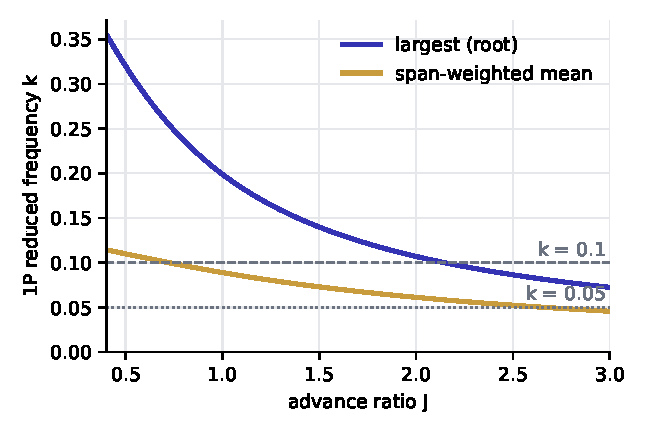
\includegraphics[width=\linewidth]{figures/qsteady_k_vs_J.pdf}
\end{column}
\begin{column}{0.49\textwidth}
\centering
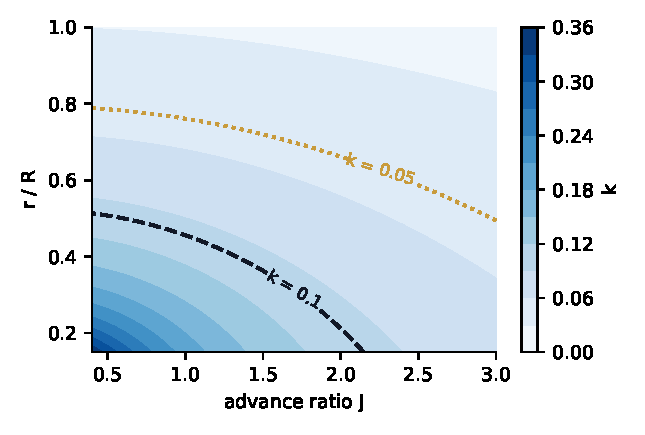
\includegraphics[width=\linewidth]{figures/qsteady_k_map_J_r.pdf}
\end{column}
\end{columns}
\par\vspace{1mm}
{\ftstablesize\renewcommand{\arraystretch}{1.0}
\begin{tabular*}{\linewidth}{@{\extracolsep{\fill}}lrrrrrr@{}}
\toprule
\(J\) & 0.6 & 1.0 & 1.4 & 1.7 & 2.2 & 3.0 \\
\midrule
\(k\) largest (root) & 0.288 & 0.199 & 0.149 & 0.125 & 0.098 & 0.072 \\
span with \(k > 0.1\) [\%] & 41.5 & 36.4 & 28.0 & 19.5 & 0 & 0 \\
\bottomrule
\end{tabular*}}
\par\vspace{0.5mm}
{\tiny\color{SoftGray} The tier-3 blade of the repository (NACA 4409, \(R\) =
1.8288 m, chord over \(R\) from 0.14 at the hub to 0.06 at the tip), from its
chord law; drawn by \code{figures/qsteady\_reduced\_frequency.py}. The root
is the worst station: short radius, wide chord.\par}
\end{frame}

\begin{frame}{What \(n\)P counts: the blade's own count}
\begin{columns}[T]
\begin{column}{0.50\textwidth}
\begin{itemize}\small
  \item \textbf{\(n\)P is counted by ONE blade}: how many times that blade
        meets the same perturbation in one revolution. An angle of attack
        is 1P; a field with four lobes around the disc is 4P, for every blade
        alike.
  \item It is \textbf{not} what a fixed surface near the rotor feels: a wing
        behind it is struck each time any of the \(N\) blades passes, so it
        counts \(N\)P (blade passing).
  \item It is \textbf{not} what a balance under the whole rotor measures:
        summing \(N\) alike blades cancels every harmonic but the multiples
        of \(N\), so only \(m\,N\)P survive there [12].
\end{itemize}
\end{column}
\begin{column}{0.46\textwidth}
\centering
\begin{tikzpicture}[x=0.95cm, y=0.55cm, font=\tiny]
  \foreach \row/\lab in {0/{one blade: 1P and 3P}, -2.3/{a fixed surface: \(N\)P, \(N = 4\)}, -4.6/{the rotor balance: \(m\,N\)P only}} {
    \draw[SoftGray, ->] (0,\row) -- (4.3,\row) node[right] {\(\psi\)};
    \node[anchor=west, text=SoftGray] at (0,\row+1.05) {\lab};
  }
  \draw[CourseBlue, thick, domain=0:360, samples=90]
    plot ({\x/90}, {0.55*sin(\x) + 0.25*sin(3*\x)});
  \draw[CourseGold, thick, domain=0:360, samples=90]
    plot ({\x/90}, {-2.3 + 0.7*abs(sin(2*\x))^6});
  \draw[CourseBlue!70!black, thick, domain=0:360, samples=90]
    plot ({\x/90}, {-4.6 + 0.12*sin(4*\x)});
  \node[text=SoftGray] at (2,-5.5) {one revolution};
\end{tikzpicture}
\end{column}
\end{columns}
\end{frame}

\begin{frame}{\code{--inflow-fft}: how many clockings a custom inflow needs}
\begin{columns}[T]
\begin{column}{0.54\textwidth}
\begin{itemize}\small
  \item A plan option, for \code{qsteady\_rotor} wheel rows with a custom
        inflow: at each radius, the Fourier series in azimuth of the angle
        of attack the \textbf{blade} meets, harmonic \(n\) being \(n\)P in the
        blade's count.
  \item \(n_{95}\): the harmonics holding 95\,\% of that perturbation;
        \(k_\mathrm{eff} = n_{95}\,k_\mathrm{1P}\), reported as minimum,
        maximum, mean and the span with \(k_\mathrm{eff} > 0.1\). With the
        option the validity warning reads \(k_\mathrm{eff}\).
  \item The suggested
        \( \code{PASSAGE\_POSITIONS} \ge n_\mathrm{max}/N + 1 \),
        and a warning when the row states fewer.
\end{itemize}
\end{column}
\begin{column}{0.42\textwidth}
\begin{block}{Why \(n_\mathrm{max}/N + 1\)}
\small The wheel's total load holds only \(m\,N\)P. \(k\) uniform clockings
inside one passage average away every \(m\,N\)P with \(m\) not a multiple of
\(k\); the first one that survives is \(k\,N\)P. So the average is clean when
\(k\,N > n_\mathrm{max}\): a blade harmonic above that aliases into the
mean.
\end{block}
\end{column}
\end{columns}
\end{frame}

\begin{frame}{What to expect against \code{unsteady\_rotor}}
\relax % a body opening with a brace group would be read as the frame subtitle
{\ftstablesize\renewcommand{\arraystretch}{1.15}
\begin{tabularx}{\linewidth}{@{}P{0.16\linewidth}P{0.34\linewidth}R@{}}
\toprule
\textbf{Component} & \textbf{qsteady against unsteady} & \textbf{Why, and what moves it} \\
\midrule
\(F_x\), \(M_x\) (thrust, torque) & \textbf{larger in magnitude}: 7 to 9\,\%
  at 10\(^\circ\) steps and 3 to 6 revolutions & the steady wake is the developed
  one; the unsteady run is still approaching it, so the gap
  \textbf{shrinks} with finer time steps and more revolutions \\
\(F_z\), \(M_z\) (normal force, yawing moment) & \textbf{smaller in
  magnitude}, by roughly 8 to 20\,\% & the phase and level of the 1P blade
  load on the downgoing half of the disc: the lag a steady solve does not
  have \\
\(F_y\), \(M_y\) (side force, pitching moment) & \textbf{unreliable}: tens of
  N against a clocking noise of about 13 N, and they may flip sign & small
  resultants of large blade loads; more clockings do not close the gap \\
\bottomrule
\end{tabularx}}
\par\vspace{1mm}
{\scriptsize A six-blade research propeller at 5\(^\circ\) on 26.124 [14]. At
0\(^\circ\) the same axial gap appears (\(-7.5\,\%\) against 6 revolutions),
so it is the wake, not the angle. Use \code{qsteady\_rotor} for thrust,
torque and trends; use \code{unsteady\_rotor} for the in-plane loads.\par}
\end{frame}

\begin{frame}{The tests behind it}
\begin{columns}[T]
\begin{column}{0.60\textwidth}
{\ftstablesize\renewcommand{\arraystretch}{1.05}
\begin{tabular*}{\linewidth}{@{\extracolsep{\fill}}lrrr@{}}
\toprule
 & U, last rev & Q, 6 clockings & \((Q-U)/|U|\) \\
\midrule
\(F_x\) [N] & \(-2022.76\) & \(-2204.64\) & \(-8.99\,\%\) \\
\(F_y\) [N] & 55.36 & \(-27.09\) & opposite sign \\
\(F_z\) [N] & 320.52 & 257.75 & \(-19.6\,\%\) \\
\(M_x\) [N m] & \(-2274.67\) & \(-2433.44\) & \(-6.98\,\%\) \\
\(M_y\) [N m] & \(-54.83\) & 44.68 & opposite sign \\
\(M_z\) [N m] & \(-410.73\) & \(-345.45\) & \(+15.9\,\%\) \\
\midrule
\(C_T\), \(C_P\) & 0.2903, 0.5623 & 0.3164, 0.6015 & \(+9.0\), \(+7.0\,\%\) \\
wall time & 102.7 s & 10.8 s & \\
\bottomrule
\end{tabular*}}
\par\vspace{0.5mm}
{\tiny\color{SoftGray} U: all six blades turning, 10\(^\circ\) per step, three
revolutions, the last averaged. Q: blades still, six clockings. RPT-089
[14].\par}
\end{column}
\begin{column}{0.37\textwidth}
\begin{ftsevidence}[The time step closes the axial gap]
\scriptsize Same propeller, a later time-step study (not yet a numbered
report): at 0\(^\circ\) and 3 revolutions the axial gap is 8.4\,\% at
10\(^\circ\) per step, 6.6\,\% at 5\(^\circ\), 4.0\,\% at 2.5\(^\circ\); 3.9\,\%
at 5\(^\circ\) and 6 revolutions. At 5\(^\circ\) incidence, 5\(^\circ\) steps,
6 revolutions: \(F_x\) 3.6\,\%, \(F_z\) 11.7\,\%, \(M_z\) 8.2\,\% apart, the
side force and pitching moment still of opposite sign. No step size levelled
off.
\end{ftsevidence}
\end{column}
\end{columns}
\end{frame}

\begin{frame}{Cost, side by side}
\relax % a body opening with a brace group would be read as the frame subtitle
{\ftstablesize\renewcommand{\arraystretch}{1.15}
\begin{tabularx}{\linewidth}{@{}P{0.28\linewidth}P{0.22\linewidth}R@{}}
\toprule
\textbf{The same rotor point} & \textbf{Wall time, one launch} & \textbf{What it buys} \\
\midrule
\code{qsteady\_rotor} wheel, 6 clockings & 10.8 s & thrust and torque; in-plane
  loads as estimates \\
\code{qsteady\_rotor} wheel, 24 clockings & about 42 s & the same, the
  clocking noise below 0.5\,\% \\
\code{unsteady\_rotor}, 10\(^\circ\), 3 revolutions & 102.7 s & the history,
  every component, a wake still developing \\
\code{unsteady\_rotor}, 5\(^\circ\), 6 revolutions & about 18 min & the axial
  gap to the steady wake down to about 4\,\% \\
\bottomrule
\end{tabularx}}
\par\vspace{1.5mm}
\begin{takeaway}Seconds against minutes: sweep \(J\), the angle and the
geometry with \code{qsteady\_rotor}, then confirm the points that matter,
and every in-plane load, with \code{unsteady\_rotor}.\end{takeaway}
{\scriptsize Six-blade research propeller, 26.124, licence checkout included
[14]; the 18 min is the time-step study of the previous frame.\par}
\end{frame}

% Copyright (c) 2026 Geovana Neves. Licensed under CC BY 4.0 (https://creativecommons.org/licenses/by/4.0/). See LICENSE-AND-AUTHORSHIP.md.
%
% 01-workspaces/text/04-running.tex

\section{Running}

\begin{frame}{Four stages}
\slidefig[0.50]{guide-stage-flow}
{\ftstablesize
\begin{tabular}{@{}lll@{}}
\toprule
\textbf{Stage} & \textbf{Windows} & \textbf{Cluster} \\
\midrule
\pyfs{plan}    & required, no seat & required, no queue \\
\pyfs{run}     & solves, then returns & submits, returns at once, \code{SUBMITTED} \\
\pyfs{collect} & not needed & waits for settled outputs, judges them \\
\pyfs{post}    & rebuilds the products & the same \\
\bottomrule
\end{tabular}}
\end{frame}

\begin{frame}{One matrix, any build}
\relax
\small
\begin{tabular}{@{}lllll@{}}
\toprule
 & 25.000 & 25.100, 26.000 & 26.100 & 26.101 and later \\
\midrule
\code{steady} & refused & runs & runs & runs \\
\code{unsteady} & refused & single march & single march & single march, or actions \\
\code{unsteady\_rotor} & refused & Euclidean rotor & unmarked, rev/min & rotary, or actions \\
\bottomrule
\end{tabular}

\vspace{2mm}
\begin{itemize}
  \item Only \code{FS\_BUILD} changes. Actions exist from 26.122.
  \item Without actions: \code{WALLTIME}, the snapshot thresholds and
  \code{FINISH\_PENDING}/\code{ADDITIONAL\_REVS} are \textbf{refused by name} at plan.
  \item \code{march\_strategy} in \code{plan.json}, the record and the superfile.
  \item A preset or pproc file can still block an older build: \textbf{plan first}.
\end{itemize}
\end{frame}

\begin{frame}{Tip and helical Mach, on every rotor point}
\[ \Omega = \frac{2\pi\,\mathrm{RPM}}{60}, \qquad
   M_\mathrm{tip} = \frac{\Omega R}{a}, \qquad
   M_\mathrm{hel} = \frac{\sqrt{V^2 + (\Omega R)^2}}{a} \]
\begin{itemize}\small
  \item For each rotor an \code{unsteady\_rotor} or \code{qsteady\_rotor} row
        turns, a \code{steady} row that states \code{RPM}, and each actuator
        disc a row names. \(R\)
        is the rotor's half diameter or the disc's tip radius; \(V\) and
        \(a\) are the point's own resolved free stream and speed of sound.
  \item \pyfs{plan} prints both per rotor and per point, and \textbf{warns},
        naming the point, when \(M_\mathrm{hel} \ge 1\): the tip is sonic or
        supersonic, where the linearised compressibility of a panel method
        stops holding [4, 12, 13]. A warning, never a refusal.
  \item The rotor table ends with \code{MTIP\_<alias>} and
        \code{MHEL\_<alias>}. Both are geometric: \(V\) is the free stream
        alone, without the rotor's own induced velocity.
\end{itemize}
\end{frame}

\begin{frame}{\pyfs{run}, on each machine}
\begin{columns}[T]
\begin{column}{0.48\textwidth}
\begin{block}{Windows}
\begin{itemize}\small
  \item A steady angle sweep is \textbf{one job over all its points}; each
        point starts cold. \code{COLD\_START: false} starts each point from
        the previous one.
  \item \code{WALLTIME} arms a clock; a run it stopped is
        \code{WALLTIME\_REACHED}, \textbf{not a failure}.
\end{itemize}
\end{block}
\end{column}
\begin{column}{0.48\textwidth}
\begin{block}{Cluster}
\begin{itemize}\small
  \item An unsteady point is \textbf{its own job}, in its own datapoint folder
        with its descriptor, action program and clock.
  \item A steady angle sweep is one job; a flow-variable sweep is one per point.
  \item A point already queued is refused a second submission. Collect it
        first.
\end{itemize}
\end{block}
\end{column}
\end{columns}
\end{frame}

\begin{frame}[fragile]{\pyfs{collect} watches the workspace, not the scheduler}
\begin{lstlisting}[style=ftsbase]
pyfs-matrix collect --workspace .            # one sweep, what a cron wants
pyfs-matrix collect --workspace . --watch    # loop until nothing is outstanding
*/15 * * * *  cd <study> && $FTS/py-venv/(*@\envname@*)/bin/pyfs-matrix collect --workspace .
\end{lstlisting}
\begin{columns}[T]
\begin{column}{0.48\textwidth}
\begin{block}{Settled is two signals}
\small Size and time stable across two looks, \textbf{and} the log present,
because the log is declared last.
\end{block}
\end{column}
\begin{column}{0.48\textwidth}
{\ftstablesize
\begin{tabular}{@{}cl@{}}
\toprule
\textbf{Exit} & \textbf{Meaning} \\
\midrule
0 & everything settled and collected \\
1 & a point it could not complete \\
3 & still outstanding \\
\bottomrule
\end{tabular}}
\end{column}
\end{columns}
\end{frame}

\begin{frame}{\code{RESTART}: continuing a march that stopped}
% \relax first: a brace group right after the title is read as a subtitle.
\relax
{\ftstablesize
\begin{tabular}{@{}ll@{}}
\toprule
\textbf{Write in the free cell} & \textbf{When} \\
\midrule
\code{RESTART: \{FINISH\_PENDING\}}     & a run the \emph{clock} stopped \\
\code{RESTART: \{ADDITIONAL\_ITERS=n\}} & any continuable run, $n$ more steps \\
\code{RESTART: \{ADDITIONAL\_REVS=n\}}  & any continuable run, $n$ more revolutions \\
\bottomrule
\end{tabular}}
\vspace{3mm}
\begin{itemize}
  \item You write \code{RESTART} and nothing else; the manifest says which run
        and how many steps are left. The count is a \textbf{remainder}.
  \item It continues the point's \textbf{most recent} run. A finished point is
        refused; a failed continuation is not retried.
  \item What it replaces is archived first, under a day and hour stamp.
\end{itemize}
\begin{takeaway}On the cluster this is the ordinary case: the queue enforces
the wall clock, so \code{\{FINISH\_PENDING\}} is the form you will use most.\end{takeaway}
\end{frame}

\begin{frame}[fragile]{Points already run, and a Linux run kept local}
\begin{lstlisting}[style=ftsbase]
pyfs-matrix run matriz.fs --workspace . --resume
pyfs-matrix run matriz.fs --workspace . --force-rerun '<point name or run id>'
pyfs-matrix run matriz.fs --workspace . --local
\end{lstlisting}
\begin{itemize}\small
  \item A recorded point is refused before anything runs; \pyfs{plan} marks it
        \code{ALREADY\_RECORDED}.
  \item \code{--resume}: only the new points of a matrix that grew.
  \item \code{--force-rerun}: redo a named point; its old record and outputs
        move to \code{archive/}, nothing is deleted. Plan again first.
        Not together with \code{--resume}.
  \item \code{--local}: on Linux with a profile, run here instead of
        submitting; the record says \code{forced\_local}. Elsewhere it changes
        nothing.
\end{itemize}
\begin{alertblock}{Redo on purpose}
\small A recorded point is never solved again by \code{--resume}. A point
whose inputs were wrong is redone by name with \code{--force-rerun}.
\end{alertblock}
\end{frame}

\begin{frame}[fragile]{The additional post}
\begin{lstlisting}[style=ftsbase]
ADDITIONAL_PPROC: p002                        # free cell; the run is unchanged
pyfs-matrix post matriz.fs --workspace . --additional-pproc
\end{lstlisting}
\begin{columns}[T]
\begin{column}{0.50\textwidth}
{\ftstablesize
\begin{tabular}{@{}ll@{}}
\toprule
\textbf{Reopened \code{.fsm}, no solve} & \textbf{Measured [3]} \\
\midrule
total loads, surface, sections & identical \\
sectional loads & identical once computed \\
unsteady plots history & identical \\
probe points off the body & \alert{not identical} \\
\bottomrule
\end{tabular}}
\end{column}
\begin{column}{0.46\textwidth}
\begin{itemize}\small
  \item Opens a copy, cuts the sections, exports, closes. Never solves or saves.
  \item \code{p002} may ask sections, their loads and the surface only.
  \item 26.124 only. Unsteady: the last instant.
  \item On the cluster: submitted, recorded \code{SUBMITTED};
        \pyfs{collect} records \code{EXTRACTED}.
\end{itemize}
\end{column}
\end{columns}
\end{frame}

\section{What a run leaves}

\begin{frame}{A simulation folder}
\begin{columns}[c]
\begin{column}{0.58\textwidth}
\slidefig[0.88]{guide-sims-anatomy}
\end{column}
\begin{column}{0.40\textwidth}
\begin{itemize}\small
  \item \code{inputs/}: a link to the mesh's library folder.
  \item \code{scripts/}: what the solver was handed. The fastest answer to
        \emph{what did this run really do}.
  \item \code{profiles/}: where the probes were placed.
  \item \code{datapoints/DP-<tag>/}: one folder per point.
\end{itemize}
\begin{takeaway}Nothing here is edited. Everything here is reproducible from
the inputs.\end{takeaway}
\end{column}
\end{columns}
\end{frame}

\begin{frame}{Inside a datapoint: what can be deleted}
% \relax first: a brace group right after the title is read as a subtitle.
\relax
{\ftstablesize
\begin{tabular}{@{}lll@{}}
\toprule
\textbf{File} & \textbf{Holds} & \textbf{Read afterwards by} \\
\midrule
\code{<stem>.fsm}         & saved simulation & \code{RESTART}. Delete it and the point cannot continue \\
\code{<stem>.txt}         & loads            & \code{polars/}, \code{campaign\_sweep.csv}, the judge \\
\code{<stem>\_sloads.txt} & sectional loads  & \code{sections/} \\
\code{<stem>\_probes.txt} & probe samples    & \code{probes/} \\
\code{<stem>\_plots.txt}  & per-step plots (unsteady) & polar, rotor averages, reductions \\
\code{<stem>\_cp.txt}, \code{<stem>.dat} & section pressures, Tecplot & nothing: a viewer \\
\code{<stem>\_log.txt}    & solver log       & \code{collect}; the first file to open \\
\bottomrule
\end{tabular}}
\vspace{2mm}
\small The stem is \code{P<POL>-<point name>}, for example
\code{P6112-M200AL+020BE+000}; the name follows the declared condition keys.
\end{frame}

\begin{frame}{Eight states, and four are not failures}
\begin{columns}[T]
\begin{column}{0.48\textwidth}
{\ftstablesize
\begin{tabular}{@{}ll@{}}
\toprule
\textbf{Not a failure} & \\
\midrule
\code{CONVERGED}           & reached its criterion \\
\code{COMPLETED\_MAX\_ITER} & reached its cap \\
\code{WALLTIME\_REACHED}    & clock stopped it \\
\code{SUBMITTED}           & in the queue \\
\bottomrule
\end{tabular}}
\end{column}
\begin{column}{0.48\textwidth}
{\ftstablesize
\begin{tabular}{@{}ll@{}}
\toprule
\textbf{Failure} & \\
\midrule
\code{FAILED\_DIVERGED}           & diverged \\
\code{FAILED\_EXECUTION}          & solver did not run \\
\code{FAILED\_SCRIPT}             & script rejected \\
\code{FAILED\_INCOMPLETE\_OUTPUT} & outputs missing \\
\bottomrule
\end{tabular}}
\end{column}
\end{columns}
\vspace{3mm}
\begin{takeaway}\code{WALLTIME\_REACHED} and \code{COMPLETED\_MAX\_ITER} carry real
numbers, and are read wrongly more often than any real failure.\end{takeaway}
\end{frame}

\section{What post-processing leaves}

\begin{frame}{Who writes the products}
\slidefig[0.42]{guide-post-anatomy}
{\ftstablesize
\begin{tabular}{@{}ll@{}}
\toprule
\pyfs{run}     & at its end, unless it submitted; no flag turns it off \\
\pyfs{collect} & after a sweep that collected something, and only then; \code{--no-post} \\
\pyfs{post}    & when you ask; no seat, no solver \\
\bottomrule
\end{tabular}}
\vspace{1mm}

\small All three \textbf{archive} what they replace, into
\code{archive/<day and hour>/}. Only \code{--force-overwrite} keeps no copy, and it
asks first. It is not part of a routine. \code{series/} is archived too.
\end{frame}

\begin{frame}{The five product folders}
% \relax first: a brace group right after the title is read as a subtitle.
\relax
{\ftstablesize
\begin{tabular}{@{}p{0.16\linewidth}p{0.50\linewidth}p{0.26\linewidth}@{}}
\toprule
\textbf{Folder} & \textbf{Answers} & \textbf{Plot against} \\
\midrule
\code{polars/}     & what the coefficients do as the condition changes; one file per group,
                     body, stability and wind axes & \code{ALPHA} or \code{BETA} \\
\code{series/}     & how it got there: loads, sections and probes per step & \code{azimuth\_deg} \\
\code{sections/}   & sectional loads, in each declared frame & \code{Offset} \\
\code{probes/}     & the flow samples, and time-average, phase-locked, per-blade reductions & \code{STEP}, \code{AZIMUTH}, \code{BLADE} \\
\code{provenance/} & inputs, script, outputs with sha256, argv, build & makes a plot defensible \\
\bottomrule
\end{tabular}}
\vspace{3mm}
\begin{itemize}\small
  \item A rotor row reduces \textbf{per rotor}: \code{<point>\_per\_blade\_<ALIAS>.csv}.
  \item In \code{campaign\_sweep.csv}, check \code{fs\_build} first: the build
        the solver reported.
\end{itemize}
\end{frame}

\begin{frame}{\code{additional/}, and what the products hold}
\begin{itemize}\small
  \item \code{post/<matrix>/additional/<pid>/}: the additional post's polars,
        sections and, unsteady, plots reductions. Every \code{products.json}
        entry says \code{"additional": true}, \code{pproc},
        \code{extraction}, \code{derives\_from}; filter on it.
  \item Its sections table keeps the run's rows first, then the new ones;
        \code{leading\_sections} counts the run's.
  \item An induced drag nobody computed is \code{NA}, with the axis columns it
        reaches. A steady probe line is exported once.
  \item Unsteady \code{series/<point>\_loads\_series.csv}: moments about the
        moment point.
  \item \code{post.log.json} beside \code{post.log}. Post a workspace with
        the package version that ran it.
\end{itemize}
\end{frame}

\begin{frame}{Vector loads and window averages}
\begin{itemize}\small
\item Steady polar axes use the exported force and moment vectors.
\code{CDB = Cx}, \code{CLB = Cz}; sideslip points get rows.
\item \code{CLS}/\code{CLW} fall by 0.10 to 0.25 per cent on 27 of 28 recorded
lifting exports, including zero sideslip; one differs by 0.71 per cent.
The cause of the export's lift discrepancy is unknown.
\item Unsteady rotor tables are window averages of all six global
\code{MRP} components over exactly the rotor's families. Missing history is a
skip, never a last-step fallback. A run adds \code{ROTOR\_<ALIAS>} if needed.
\item \code{RPM\_<alias>} and \code{DIAMETER\_<alias>} join the rotor header;
\code{J\_<alias>} uses the free stream. $\mathrm{ETAW}=J\,\mathrm{CTW}/\mathrm{CP}$
uses the whole force in wind axes and equals \code{ETA} along the stream.
\item \code{ETAW} and the shaft angle follow the stream direction at
incidence or sideslip; a re-post needs no solver.
\end{itemize}
\end{frame}

\begin{frame}{Read columns by name}
\begin{itemize}\small
\item Condition: \code{ALPHA, BETA, MACH, RE, VINF, VREF, ALT, RHO, TEMP, MU,}
\code{J, SREF, CREF, BREF}. Plots keep the export's own headings.
\item Unsteady polar: \code{P<sim>\_<name>\_uns\_avg.csv}, beginning with
\code{FIRST\_STEP, LAST\_STEP, STEPS}; adds moment point, group-suffixed axes,
equations and super-file content.
\item Axes need all six global \code{MRP} plots. A new run supplies
\code{MRP\_TOTAL} if absent; a history without them has a \code{\#axes} skip.
\item Reductions carry \code{ROTOR} and \code{XMOM, YMOM, ZMOM}, not
\code{Time-step} and \code{Time (sec)}.
\item Sections: \code{STEP, FAMILY, PLANE, ROTOR, AZIMUTH}; still one instant.
Azimuth is blade one of that row's rotor, or \code{NA} without one.
\item Series use \code{STEP}, add the condition block; probes add \code{PROBE}.
\end{itemize}
\end{frame}

\begin{frame}{One row per blade, or per azimuth}
\begin{itemize}\small
\item \code{per\_blade}: one row per blade, each blade's own rotor clock and matrix window,
\code{BLADE, FAMILY, AZIMUTH\_START, AZIMUTH\_END}. A blade's family suffix is
removed from its own plot columns so all blades share headings.
\item Declared \code{[phase\_locked]}: one row per azimuth of the last
revolution, averaged across the requested revolutions. Blade columns align by
each blade's own azimuth; other columns use blade one.
\item The row's total revolutions must be \emph{at least}
\code{min\_revolutions}. A shorter run loses only that table. Without the
pproc declaration, the file remains a passage series.
\item Editing the matrix window moves the reductions together at post;
editing the pproc gate or depth also needs no new solver run. Records stay as written.
\item Read \code{products.json}: \code{complete}, \code{interrupted}, sources,
windows and skips. \code{\#axes}, \code{\#equations}, \code{\#names} count for
\code{post --strict} even if the rest of the file was written.
\end{itemize}
\end{frame}

\begin{frame}{Collection and manifest limits}
\begin{itemize}
\item An early export at an iteration-limit run, confirmed by the solver log,
and a velocity mismatch are failures and leave the products.
\item A continuation's \code{continues} field excludes its predecessor from
products and the sweep table.
\item Stamped series exports are found in both simulation and datapoint
folders; a missing kind is a skip, not a header-only product.
\end{itemize}
\begin{alertblock}{Manifest ownership}
A live writer renews its owned lock every 5 seconds. Takeover requires a dead
local owner or a heartbeat older than 300 seconds. Finish every older writer
before a newer one uses the same workspace.
\end{alertblock}
\end{frame}

\begin{frame}{Reading a result honestly}
\begin{itemize}
  \item For unsteady, \code{CONVERGED} checks the last time step's inner
        iterations. Whether the history has settled is the user's judgement.
        It does not mean the mesh was
        fine, the reference right, or the physics the one you meant.
  \item A curve that stops early at \code{WALLTIME\_REACHED} is real up to that
        step. Continue it, do not repeat it.
  \item One diverged point in a swept row is judged on its own.
\end{itemize}
\begin{ftslimit}
The workspace makes a study reproducible and traceable. That is not the same
as correct, and no amount of green status is evidence of the second.
\end{ftslimit}
\end{frame}

\begin{frame}{Re-posting a recorded campaign}
\begin{itemize}\small
  \item Run \code{pyfs-matrix post --workspace <root>} without a solver.
        Records remain unchanged; each product is written or skipped with its reason.
  \item Nothing blocks by default: frozen-solve averages are
        WARNED in \code{post.log} and written; \code{--check-frozen} withholds
        them. The unsteady polar's \code{ADVANCE\_RATIO} states the point's \code{J}.
  \item Every unsteady probe uses fluid plots. A cited profile recorded only
        as an instant needs a new run for its missing history.
  \item Each distribution gains \code{\_sloads\_<name>.csv} and
        \code{\_cp\_<name>.csv}, with every available exported \code{STEP}.
  \item New VTK/CSV exports and the pproc surface-averaging window need a new
        solver run. Guides 4 and 5 have the keys [4].
  \item \code{integrate = true} on a sections entry adds the
        strip force and moment columns on re-post, without a solver run.
\end{itemize}
\end{frame}

% Copyright (c) 2026 Geovana Neves. Licensed under CC BY 4.0 (https://creativecommons.org/licenses/by/4.0/). See LICENSE-AND-AUTHORSHIP.md.
%
% 01-workspaces/text/06-two-workspaces-sync.tex
%
% Working on a Windows workstation and on an HPC cluster: two workspaces, one
% of them the main, kept together by pyfs-matrix sync. Source of record:
% docs/storage-and-sync.md and `pyfs-matrix sync --help` of the version on
% the title page.

\section{Windows and an HPC cluster: two workspaces and sync}
\label{sec:two-workspaces}

\begin{frame}{Two workspaces, one of them the main}
\begin{columns}[T]
\begin{column}{0.48\textwidth}
\begin{block}{The main workspace, on Windows}
\begin{itemize}\small
  \item {\scriptsize\code{\mainworkspace}}: \textbf{the reference}. Its \code{runs.json},
        its \code{post/} and its matrices are the record everybody reads.
  \item It is the one under version control.
  \item Runs can be done here: planning, one point, a steady sweep.
\end{itemize}
\end{block}
\end{column}
\begin{column}{0.48\textwidth}
\begin{block}{The cluster workspace}
\begin{itemize}\small
  \item Where runs are \textbf{submitted} to the queue and collected:\\
        {\scriptsize\code{\clusterworkspace}}.
  \item The same \code{inputs/} library as the main: references, setups,
        pproc files, geometries.
  \item Its own matrices, its own \code{sims/} and \code{runs.json}.
\end{itemize}
\end{block}
\end{column}
\end{columns}
\begin{takeaway}Runs are done in either workspace. \pyfs{pyfs-matrix sync}, run
on the main, brings the cluster's runs and results home.\end{takeaway}
\end{frame}

\begin{frame}{How they relate}
\begin{center}
\begin{tikzpicture}[font=\scriptsize,
  w/.style={draw=CourseBlue, thick, rounded corners, fill=CourseBlue!8,
            align=center, text width=46mm, minimum height=22mm, inner sep=3pt},
  lib/.style={draw=CourseGold, thick, rounded corners, fill=CourseGold!15,
              align=center, text width=34mm, minimum height=10mm, inner sep=3pt}]
\node[w] (main) {\textbf{main workspace} (Windows)\\[2pt]
  owns \code{matriz.fs}\\ \code{runs.json}, \code{post/}, \code{sims/}\\
  \tiny\code{inputs/sync-workspaces.toml}};
\node[w, right=36mm of main] (hpc) {\textbf{cluster workspace}\\[2pt]
  owns \code{matriz\_hpc.fs}\\ \code{runs.json}, \code{post/}, \code{sims/}\\
  \tiny\code{inputs/hpc/h001.toml}};
\node[lib, below=8mm of $(main)!0.5!(hpc)$] (inputs) {the same \code{inputs/}\\ \tiny references, setups, pproc, geometries};
\draw[-{Stealth}, very thick, CourseGreen] (hpc.west) -- node[above, font=\tiny] {\code{sync runs | post | fsm | all}} node[below, font=\tiny] {preview, then \code{--apply}} (main.east);
\draw[CourseGold, thick] (inputs) -- (main.south);
\draw[CourseGold, thick] (inputs) -- (hpc.south);
\end{tikzpicture}
\end{center}
\begin{itemize}\small
  \item \textbf{Every matrix is owned by exactly one workspace.} The owner
        edits it; the other only receives it.
  \item \pyfs{sync} runs \textbf{on the main} and pulls. It never writes into
        the cluster workspace.
\end{itemize}
\end{frame}

\begin{frame}[fragile]{\code{inputs/sync-workspaces.toml}}
\begin{columns}[T]
\begin{column}{0.60\textwidth}
\begin{lstlisting}[style=ftsbase]
main = "windows"

[workspaces.windows]
path = "."
matrices = ["matriz"]

[workspaces.cluster]
path = "(*@\clusterworkspaceunc@*)"
matrices = ["matriz_hpc"]
\end{lstlisting}
\end{column}
\begin{column}{0.37\textwidth}
\begin{itemize}\small
  \item \code{main} names the entry you stand in; \pyfs{sync} is run there.
  \item One \code{[workspaces.<name>]} table per workspace: its \code{path}
        (as the main sees it) and the \code{matrices} it \textbf{owns}, by
        stem.
  \item A stem declared by two workspaces refuses the sync, and so does a
        matrix file that no workspace declares.
  \item \code{--from cluster} pulls from one workspace; without it, from
        every other one.
\end{itemize}
\end{column}
\end{columns}
\end{frame}

\begin{frame}[fragile]{Four levels, each one the previous plus more}
\begin{lstlisting}[style=ftsbase]
pyfs-matrix sync post --workspace .            # preview: changes nothing
pyfs-matrix sync post --workspace . --apply    # then do it
\end{lstlisting}
{\ftstablesize
\begin{tabular}{@{}lp{0.78\linewidth}@{}}
\toprule
\textbf{Level} & \textbf{Brings} \\
\midrule
\code{runs} & the records in \code{runs.json}, and the provenance each needs to be believed: every simulation's \code{scripts/} and its datapoint logs \\
\code{post} & the above, plus the \code{post/} folder, its products and their provenance \\
\code{fsm}  & the above, plus the saved simulation of every datapoint \\
\code{all}  & the above, plus everything else under \code{sims/} \\
\bottomrule
\end{tabular}}
\vspace{2mm}
\begin{takeaway}Every call previews by default and changes files only with
\code{--apply}. Read the preview first.\end{takeaway}
\end{frame}

\begin{frame}{How a conflict is settled}
\begin{columns}[T]
\begin{column}{0.48\textwidth}
\begin{block}{Run records and files}
\begin{itemize}\small
  \item Only in the other workspace: added. Identical: left alone.
  \item Different: if main's record is still \code{SUBMITTED}, the other's
        wins; otherwise \textbf{main wins} unless \code{--prefer-other}.
  \item A file in both with different content: main's copy stays unless
        \code{--overwrite}, which archives it to
        \code{archive/sync-<stamp>/} first.
\end{itemize}
\end{block}
\end{column}
\begin{column}{0.48\textwidth}
\begin{alertblock}{Matrices: ownership decides}
\small Any difference between main's copy and the source's is reported as a
\textbf{MERGE CONFLICT}, every time, and \textbf{the owner's copy wins}. When
the source owns it, main's copy is archived and replaced; when main owns it,
main's copy stays. \code{--prefer-other} and \code{--overwrite} do not apply
to matrices.
\end{alertblock}
\end{column}
\end{columns}
\end{frame}

\begin{frame}{What sync never does}
\begin{itemize}\small
  \item \textbf{It never copies a mesh.} A synced simulation's \code{inputs}
        is linked again into the main's own \code{inputs/geometries/}, to the
        same geometry folder. A geometry the main library lacks is not
        linked, and the sync says so.
  \item \textbf{A run still \code{SUBMITTED} there syncs its record only}:
        nothing finished is worth copying, and a job may still be writing.
  \item It deletes nothing in the main and never touches \code{inputs/},
        except a declared matrix.
  \item It never brings back a run id that \pyfs{delete-sims} retired in the
        main.
  \item \code{runs.json} is archived before it is rewritten. A lock in the
        main (a run in progress) refuses the sync; a lock in a source skips
        that source, with the reason.
\end{itemize}
\begin{takeaway}Every call, one entry per source workspace, is recorded in
\code{storage\_management.json} at the main's root.\end{takeaway}
\end{frame}

\begin{frame}[fragile]{A routine that works}
\begin{enumerate}\small
  \item On the main: edit and plan the matrices it owns; commit them.
  \item Bring the cluster's \code{inputs/} up to date from the main (the
        site's copy procedure), before planning there.
  \item On the cluster: plan, run (it submits), \pyfs{collect} until
        nothing is outstanding. Edit only the matrices the cluster owns.
  \item On the main, in Windows:
\begin{lstlisting}[style=ftsbase]
pyfs-matrix sync post --workspace .          # read the preview
pyfs-matrix sync post --workspace . --apply
\end{lstlisting}
  \item Commit the synced matrices on the main, with the reason.
\end{enumerate}
\end{frame}

\section{Space on disk}
\label{sec:storage}

\begin{frame}[fragile]{Three commands that keep a workspace small}
\begin{lstlisting}[style=ftsbase]
pyfs-matrix space-in-use --workspace .              # sizes; changes nothing
pyfs-matrix free-space m001 --workspace . --apply   # inputs/management/m001.toml
pyfs-matrix delete-sims 4001,2009 --workspace . --apply
\end{lstlisting}
\begin{itemize}\small
  \item \code{space-in-use}: sizes by top folder, by \code{sims/sim\_*} and by
        extension (\code{--top N}).
  \item \code{free-space}: compacts simulation folders into
        \code{sims/sim\_<id>.zip}, deletes files of named extensions, compacts
        or deletes \code{post/<matrix>/archive/}. A compacted folder is
        restored, hash checked, the moment \pyfs{post}, \pyfs{collect} or a
        continuation needs it.
  \item \code{delete-sims}: a simulation, its own products and its records;
        a product shared with other points needs \code{--matrix-products}.
  \item The \code{.fsm}, \code{scripts/}, logs and every file a record names
        are never deleted; neither is the mesh, whose link is undone first.
        Every call is recorded in \code{storage\_management.json}.
\end{itemize}
\end{frame}

\begin{frame}{Per-step exports: keep the last step}
\begin{columns}[T]
\begin{column}{0.52\textwidth}
\begin{itemize}\small
  \item An unsteady point that exports along its march (the surface of an
        averaging window, the stamped series) leaves one file per step. They
        are the largest thing a campaign keeps.
  \item A \code{free-space} mode deletes them and \textbf{keeps only the last
        step's} export of each unsteady point. Like every storage call it
        previews first and deletes only with \code{--apply}, and the call is
        recorded.
  \item Products already written stay as they are.
\end{itemize}
\end{column}
\begin{column}{0.44\textwidth}
\begin{alertblock}{A later post that needs a deleted step}
\small is \textbf{refused}, naming the point and the step that is gone.
Nothing is averaged over a window with holes in it. Post everything a
campaign needs before freeing its steps, or run the point again.
\end{alertblock}
\end{column}
\end{columns}
\end{frame}

% Copyright (c) 2026 Geovana Neves. Licensed under CC BY 4.0 (https://creativecommons.org/licenses/by/4.0/). See LICENSE-AND-AUTHORSHIP.md.
%
% 01-workspaces/text/05-vcs-and-reference.tex

\section{Version control}
\label{sec:slides-vcs}

\begin{frame}{What version control carries}
\begin{columns}[T]
\begin{column}{0.48\textwidth}
{\ftstablesize
\begin{tabular}{@{}p{0.32\linewidth}p{0.58\linewidth}@{}}
\toprule
\textbf{In} & \textbf{Why} \\
\midrule
the matrices     & the study; written, not produced \\
\code{inputs/}   & every file a row cites \\
\code{ansa/}     & the script encodes the decision \\
\code{docs/}     & a second person needs it \\
\code{builds/}   & a site decision: a checkout is complete \\
\bottomrule
\end{tabular}}
\end{column}
\begin{column}{0.48\textwidth}
{\ftstablesize
\begin{tabular}{@{}p{0.54\linewidth}p{0.36\linewidth}@{}}
\toprule
\textbf{Out} & \textbf{Why} \\
\midrule
\code{executables.local.toml} & true of one machine only \\
the meshes                     & large, derived from \code{ansa/} \\
\code{sims/}, \code{post/}, \code{archive/} & produced \\
\code{pfs-wheels/}, \code{py-venv/} & binaries, absolute paths \\
\bottomrule
\end{tabular}}
\end{column}
\end{columns}
\begin{takeaway}Version inputs, not run products. The generated \code{VARIABLES.md} and
\code{WRITING-EQUATIONS.md} in pproc may be committed or ignored.\end{takeaway}
\end{frame}

\begin{frame}{Version control lives with the main workspace}
\begin{columns}[T]
\begin{column}{0.50\textwidth}
\begin{itemize}\small
  \item \textbf{The main workspace is the checkout.} The cluster workspace
        holds a copy of its \code{inputs/}, not a checkout.
  \item Every matrix of the study is in version control, whichever workspace
        owns it: \pyfs{sync} brings the cluster's matrices to the main, where
        they are committed.
  \item \pyfs{plan} checks every POL against \textbf{every} \code{.fs} of the
        workspace it runs in.
\end{itemize}
\end{column}
\begin{column}{0.46\textwidth}
\begin{alertblock}{Why a stale copy lets a collision through}
\small \code{--update-ids} picks the next free POL from the matrices, run
records and \code{sims/} \textbf{of its own side}. A POL used only on the
cluster is invisible on the main until a sync brings its matrix, and the
cluster sees a new main row only once its inputs are refreshed.
\end{alertblock}
\end{column}
\end{columns}
\end{frame}

\begin{frame}{The ritual that keeps \pyfs{plan} honest}
\begin{enumerate}\small
  \item \textbf{Update} the main checkout, and \textbf{sync} it from the
        cluster, before touching any matrix.
  \item \textbf{Edit and plan the main's matrices on the main}, where every
        matrix sits side by side, so a repeated POL is refused there.
  \item \textbf{Commit} at once, with the reason in the message.
  \item \textbf{Refresh the cluster's inputs} from the main before planning
        or running there.
  \item \textbf{Edit a cluster-owned matrix only on the cluster}, and bring it
        home with the next sync; commit it on the main before its results are
        used.
\end{enumerate}
\begin{takeaway}The main workspace is the one place every matrix meets. A plan
run anywhere else is only as right as the last refresh.\end{takeaway}
\end{frame}

\begin{frame}{The daily cycle, and the two commits that hurt everyone}
\begin{columns}[T]
\begin{column}{0.48\textwidth}
\begin{block}{Every day}
\begin{itemize}\small
  \item \textbf{Update and sync before you plan.}
  \item \textbf{Commit an input change with its reason}: which row, and what
        changed about the physics.
  \item \textbf{Never commit while a run is writing.}
\end{itemize}
\end{block}
\end{column}
\begin{column}{0.48\textwidth}
\begin{alertblock}{Never commit}
\begin{itemize}\small
  \item \code{sims/} after a campaign: hundreds of megabytes in every
        colleague's next update.
  \item \code{executables.local.toml}: it silently redirects everybody who
        updates.
\end{itemize}
\end{alertblock}
\end{column}
\end{columns}
\end{frame}

\section{Reference}

\begin{frame}{Refusals you will meet first}
% \relax first: a brace group right after the title is read as a subtitle.
\relax
{\ftstablesize
\begin{tabular}{@{}p{0.40\linewidth}p{0.54\linewidth}@{}}
\toprule
\textbf{Message contains} & \textbf{Do this} \\
\midrule
\code{POL(s) are stated more than once across the matrices} & renumber, or \code{plan ... --update-ids}; then commit and refresh \\
\code{cites the probe survey ... holds no such file} & put the survey in \code{inputs/profiles/} \\
\code{is already in a scheduler's queue as} & \code{pyfs-matrix collect} first \\
\code{maps no alias for build(s)} & add the build's line under \code{[builds]} \\
\code{and nothing says which cluster this machine is} & keep exactly one profile in \code{inputs/hpc/} \\
\code{the record it continues does not say where it stopped} & use \code{\{ADDITIONAL\_ITERS=n\}} \\
\code{which is not a run that STOPPED with more to do} & drop \code{RESTART}; nothing to continue \\
\code{TRANSLATE DISTANCE is ..., which is not a finite number} & write metres, as \code{0.05} \\
\code{is ignored: it is either a non-existing path} & the wheels folder is not there (Guide 7) \\
\code{bad interpreter} & the environment was moved; rebuild it in place \\
\bottomrule
\end{tabular}}
\end{frame}

\begin{frame}{Refusals to resolve before using results}
\begin{itemize}\small
\item No unsteady window: add \code{LAST\_REVS\_AVG} or
\code{LAST\_ITERS\_AVG}. \code{WINDOW\_*} keys are refused.
\item Duplicate attitude: keep \code{ALPHA}/\code{BETA} in one cell.
Duplicate stabilisation: keep one preset interface.
\item Linked file destination or names differing only by case: use ordinary,
distinct staging destinations and update references.
\item Unknown export-frame rotation: export loads in global \code{MRP}.
\item Export area/chord mismatch: reconcile the project and reference
\code{SREF}/\code{CREF}; the simulation otherwise gets no product.
\item Invalid plot name: letters, digits, underscores and bare
\code{\{family\}} only. Ambiguous names skip rotor histories or axes blocks.
\end{itemize}
\end{frame}

\begin{frame}{Forms that are refused, and what to write}
\small Each is refused naming its replacement:
\begin{itemize}\small
  \item \code{iteration=}: write \code{step=}.
  \item \code{run.assess\_unsteady\_from\_plots}: use \code{LoadsAssessor}.
  \item The three \code{WINDOW\_*} row keys: \code{LAST\_ITERS\_AVG} or
        \code{LAST\_REVS\_AVG} (degrees divided by 360).
  \item Group-member lists: one alias per group, members in the reference's
        \code{[aliases]}.
\end{itemize}
\small The \code{broken\_commands} reader stays as plain compatibility.
Existing run records are never rewritten.
\end{frame}

\begin{frame}[fragile]{Cheatsheet}
% \relax first: a brace group right after the title is read as a subtitle.
\relax
{\ftstablesize
\begin{tabular}{@{}>{\raggedright\arraybackslash}p{0.10\linewidth}
                 >{\raggedright\arraybackslash}p{0.52\linewidth}
                 >{\raggedright\arraybackslash}p{0.30\linewidth}@{}}
\toprule
\textbf{Step} & \textbf{Windows (main)} & \textbf{Cluster} \\
\midrule
get in   & \code{.venv\textbackslash Scripts\textbackslash activate} & \code{source \$FTS/bin/\envname-env} \\
get out  & \code{deactivate} & new shell, or \code{exit} \\
update   & update the checkout & refresh the inputs from the main \\
plan     & \code{pyfs-matrix plan <matrix>.fs --workspace . --fs-version 26.123} & same \\
POL fix  & \code{... --update-ids} & same, then sync and commit on the main \\
run      & \code{pyfs-matrix run <matrix>.fs --workspace . --fs-version 26.123} & same; submits \\
collect  & not needed & \code{pyfs-matrix collect --workspace .} \\
sync     & \code{pyfs-matrix sync post --workspace . --apply} & not run here \\
post     & \code{pyfs-matrix post <matrix>.fs --workspace .} & same \\
continue & \code{RESTART: \{FINISH\_PENDING\}} in the free cell & same \\
space    & \code{pyfs-matrix space-in-use --workspace .} & same \\
\bottomrule
\end{tabular}}
\vspace{2mm}

{\scriptsize \code{\$FTS} is \code{\clusterroot}.}
\end{frame}

\begin{frame}{Where to go next}
\begin{columns}[T]
\begin{column}{0.48\textwidth}
\begin{itemize}\small
  \item \textbf{The other guides}: 2, from the GUI to pyfs; 3, the reference
        file; 4, solver setup; 5, post-processing definitions; 6, FSI; 7,
        Python on an offline machine.
  \item \textbf{The package}: its own documentation [1, 2].
\end{itemize}
\end{column}
\begin{column}{0.48\textwidth}
\begin{block}{Cite the version}
\small \pkgcitation
\end{block}
\end{column}
\end{columns}
\end{frame}


\begin{frame}{References}
\begin{reflist}
  \bibitem{g01r01} \docref{workspace-and-workflows}{The workspace and the workflow}
  \bibitem{g01r02} \docref{storage-and-sync}{Storage and sync}
  \bibitem{g01r03} \recordsref
  \bibitem{g01r04} \docref{post-processing-definitions}{Post-processing definitions}
  \bibitem{g01r05} \docref{flight-conditions}{Flight conditions}
  \bibitem{g01r06} \docref{excel-matrices}{Optional Excel matrix workbook}
  \bibitem{g01r07} International Organization for Standardization, \emph{ISO
        2533:1975, Standard Atmosphere}, ISO, Geneva, 1975.
  \bibitem{g01r08} F. M. White, \emph{Viscous Fluid Flow}, 3rd ed., McGraw-Hill, New
        York, 2006. Sutherland's law for the viscosity of air.
  \bibitem{SMI} \smiref
  \bibitem{g01r10} T. Theodorsen, ``General theory of aerodynamic instability and the
        mechanism of flutter'', NACA Report 496, 1935.
\end{reflist}
\end{frame}

\begin{frame}{References (continued)}
\begin{reflist}
  \setcounter{enumi}{10}
  \bibitem{g01r11} W. R. Sears, ``Some aspects of non-stationary airfoil theory and its
        practical application'', \emph{Journal of the Aeronautical Sciences},
        8(3), pp. 104-108, 1941.
  \bibitem{g01r12} J. G. Leishman, \emph{Principles of Helicopter Aerodynamics}, 2nd
        ed., Cambridge University Press, Cambridge, 2006.
  \bibitem{g01r13} H. Glauert, ``The effect of compressibility on the lift of an
        aerofoil'', \emph{Proceedings of the Royal Society of London, Series
        A}, 118(779), pp. 113-119, 1928.
  \bibitem{g01r14} \pkgauthor, ``The quasi-steady rotor against the unsteady rotor,
        measured'', report RPT-089, 2026, \code{reports/} of \url{\pkgrepo}.
\end{reflist}
\end{frame}

\end{document}
